% Options for packages loaded elsewhere
\PassOptionsToPackage{unicode}{hyperref}
\PassOptionsToPackage{hyphens}{url}
\PassOptionsToPackage{dvipsnames,svgnames*,x11names*}{xcolor}
%
\documentclass[
  ignorenonframetext,
  aspectratio=169]{beamer}
\usepackage{pgfpages}
\setbeamertemplate{caption}[numbered]
\setbeamertemplate{caption label separator}{: }
\setbeamercolor{caption name}{fg=normal text.fg}
\beamertemplatenavigationsymbolsempty
% Prevent slide breaks in the middle of a paragraph
\widowpenalties 1 10000
\raggedbottom
\setbeamertemplate{part page}{
  \centering
  \begin{beamercolorbox}[sep=16pt,center]{part title}
    \usebeamerfont{part title}\insertpart\par
  \end{beamercolorbox}
}
\setbeamertemplate{section page}{
  \centering
  \begin{beamercolorbox}[sep=12pt,center]{part title}
    \usebeamerfont{section title}\insertsection\par
  \end{beamercolorbox}
}
\setbeamertemplate{subsection page}{
  \centering
  \begin{beamercolorbox}[sep=8pt,center]{part title}
    \usebeamerfont{subsection title}\insertsubsection\par
  \end{beamercolorbox}
}
\AtBeginPart{
  \frame{\partpage}
}
\AtBeginSection{
  \ifbibliography
  \else
    \frame{\sectionpage}
  \fi
}
\AtBeginSubsection{
  \frame{\subsectionpage}
}
\usepackage{lmodern}
\usepackage{amssymb,amsmath}
\usepackage{ifxetex,ifluatex}
\ifnum 0\ifxetex 1\fi\ifluatex 1\fi=0 % if pdftex
  \usepackage[T1]{fontenc}
  \usepackage[utf8]{inputenc}
  \usepackage{textcomp} % provide euro and other symbols
\else % if luatex or xetex
  \usepackage{unicode-math}
  \defaultfontfeatures{Scale=MatchLowercase}
  \defaultfontfeatures[\rmfamily]{Ligatures=TeX,Scale=1}
\fi
\usetheme[]{Frankfurt}
\usecolortheme{beaver}
\usefonttheme{structuresmallcapsserif}
% Use upquote if available, for straight quotes in verbatim environments
\IfFileExists{upquote.sty}{\usepackage{upquote}}{}
\IfFileExists{microtype.sty}{% use microtype if available
  \usepackage[]{microtype}
  \UseMicrotypeSet[protrusion]{basicmath} % disable protrusion for tt fonts
}{}
\makeatletter
\@ifundefined{KOMAClassName}{% if non-KOMA class
  \IfFileExists{parskip.sty}{%
    \usepackage{parskip}
  }{% else
    \setlength{\parindent}{0pt}
    \setlength{\parskip}{6pt plus 2pt minus 1pt}}
}{% if KOMA class
  \KOMAoptions{parskip=half}}
\makeatother
\usepackage{xcolor}
\IfFileExists{xurl.sty}{\usepackage{xurl}}{} % add URL line breaks if available
\IfFileExists{bookmark.sty}{\usepackage{bookmark}}{\usepackage{hyperref}}
\hypersetup{
  pdftitle={Introduction to Plant Biotechnology},
  pdfauthor={Deependra Dhakal},
  colorlinks=true,
  linkcolor=red,
  filecolor=Maroon,
  citecolor=blue,
  urlcolor=red,
  pdfcreator={LaTeX via pandoc}}
\urlstyle{same} % disable monospaced font for URLs
\newif\ifbibliography
\setlength{\emergencystretch}{3em} % prevent overfull lines
\providecommand{\tightlist}{%
  \setlength{\itemsep}{0pt}\setlength{\parskip}{0pt}}
\setcounter{secnumdepth}{-\maxdimen} % remove section numbering
\usepackage{booktabs}
\usepackage{longtable}
\usepackage{array}
\usepackage{multirow}
\usepackage{wrapfig}
\usepackage{float}
\usepackage{colortbl}
\usepackage{pdflscape}
\usepackage{tabu}
\usepackage{threeparttable}
\usepackage{threeparttablex}
\usepackage[normalem]{ulem}
\usepackage{makecell}
\usepackage{xcolor}

% % set background image if you will
% \usebackgroundtemplate%
% {%
%     \includegraphics[width=\paperwidth,height=\paperheight]{02-dna_modification_background_dna_helix.jpg}%
% }

% % set background in a TikZ node for modifications
% % set background in a TikZ node for modifications
\usepackage{tikz}
\usepackage[absolute,overlay]{textpos}
\setbeamertemplate{title page}{
\tikz\node[opacity=0.8] {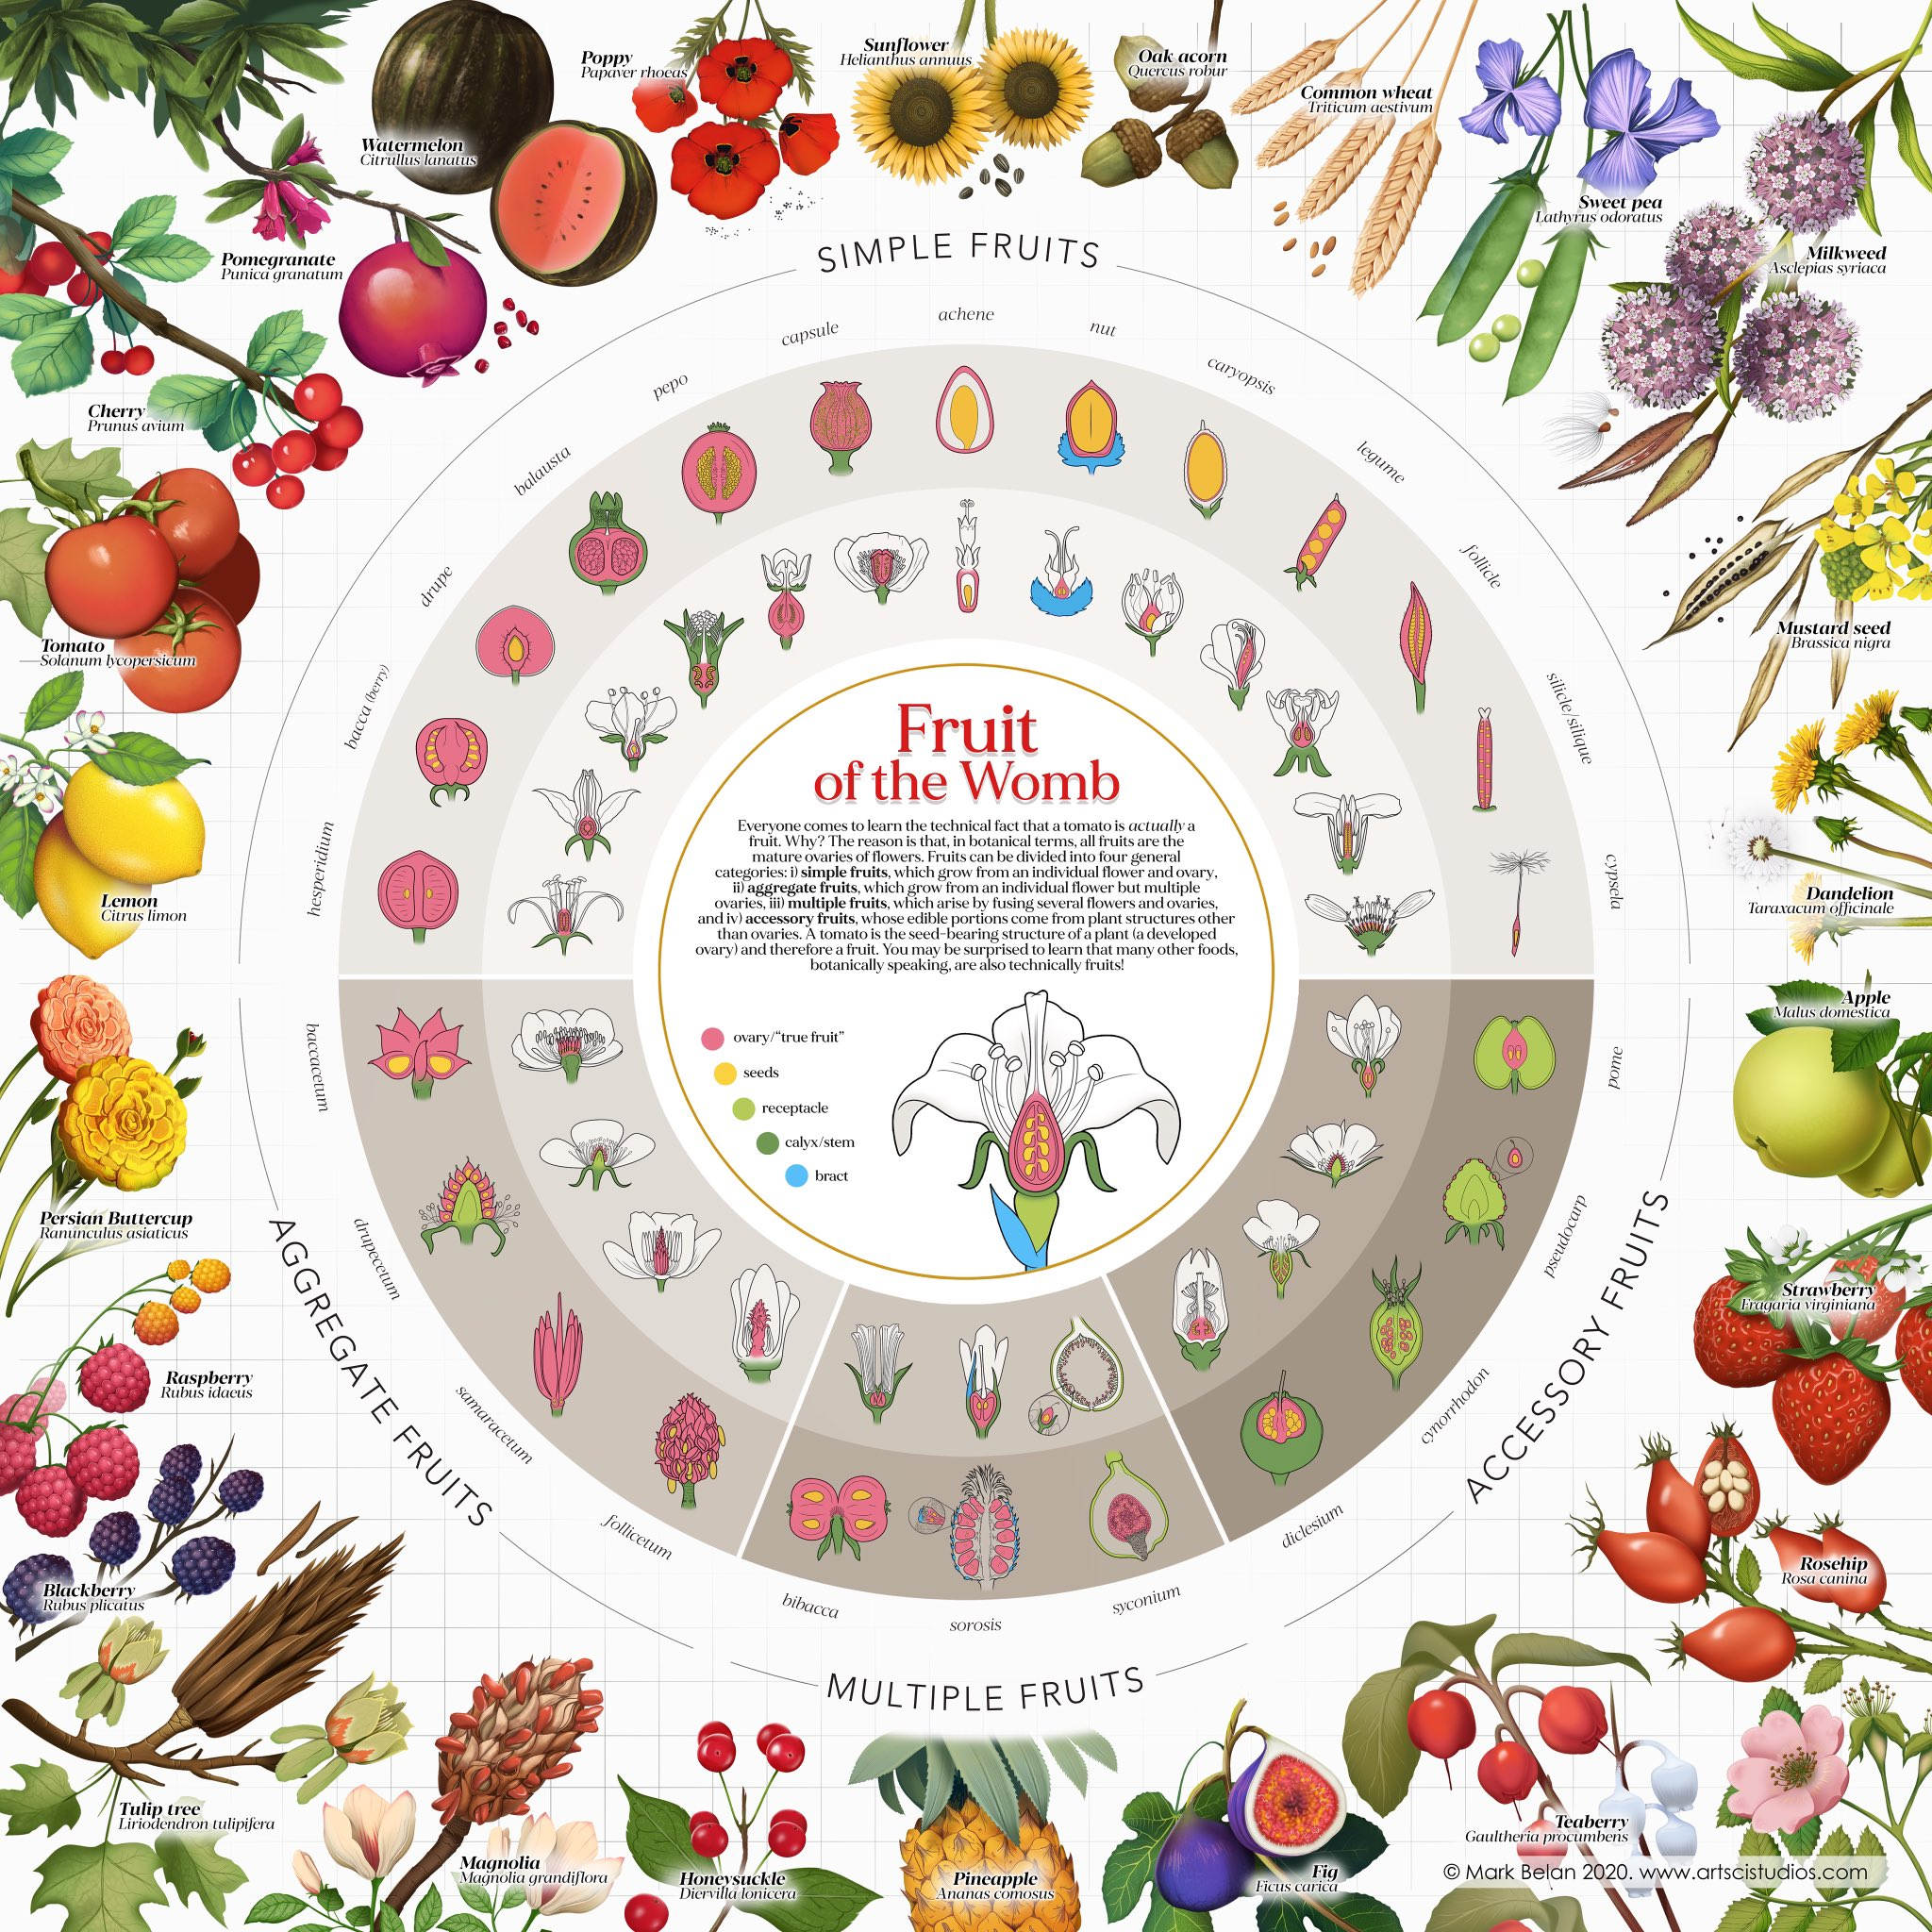
\includegraphics[width=0.8\paperwidth]{./02-fruit_of_womb.jpg}};
% \tikz\node[opacity=0.8] {\includegraphics[width=5cm,ext=.1-overview_mutation_cover.png,type=png,read=.1-overview_mutation_cover.png]{1}} % if name shall contain dots, suppose filename = 01.1-overview_mutation_cover.png
\begin{textblock}{15}(4,5)\usebeamerfont{title} % 1.5 is x position in page
{\color{black}\raggedright\par\inserttitle}\\[0.4cm]
% \end{textblock}
% \begin{textblock}{7.5}(1.5,7) % 1.5 is x position in page
{\color{black}\raggedright{\insertauthor}\mbox{}\\[0.2cm]
\insertdate}
\end{textblock}} % dd_rookie modified, figure is top aligned

% % set caption font size
% % note that beamer presentation native captions have their own configs
% \usepackage{caption}
% \captionsetup{font=footnotesize}

% this font option is amenable for beamer
\setbeamerfont{caption}{size=\tiny}

% some beamer themes naturally might not support navigation symbols
% \setbeamertemplate{navigation symbols}{} % remove navigation symbols

\setbeamertemplate{footline}[page number] % insert page number in footline

% \setbeamertemplate{navigation symbols}{slide} % insert slide indication in navigation
% \setbeamertemplate{navigation symbols}{frame} % insert frame indication in navigation
% \setbeamertemplate{navigation symbols}{section} % insert section indication in navigation
% \setbeamertemplate{navigation symbols}{subsection} % insert subsection indication in navigation

% \AtBeginSubsection{} % supress subsection display
\newlength{\cslhangindent}
\setlength{\cslhangindent}{1.5em}
\newenvironment{cslreferences}%
  {\setlength{\parindent}{0pt}%
  \everypar{\setlength{\hangindent}{\cslhangindent}}\ignorespaces}%
  {\par}

\title{Introduction to Plant Biotechnology}
\subtitle{Plant Biotechnology: Definition, history, fields}
\author{Deependra Dhakal}
\date{Academic year 2022-2023}
\institute{CNRM, Tikapur \and AFU}

\begin{document}
\frame{\titlepage}

\begin{frame}[allowframebreaks]
  \tableofcontents[hideallsubsections]
\end{frame}
\hypertarget{background}{%
\section{Background}\label{background}}

\begin{frame}{Overview}
\protect\hypertarget{overview}{}
\begin{itemize}
\tightlist
\item
  Biotechnology has been around ever since humans began manipulating the
  natural environment to improve their food supply, housing and health.
\end{itemize}

\begin{columns}[T,onlytextwidth]
  \scriptsize
  \column{0.4\textwidth}
  \begin{alertblock}{Alert}
  In 1974, a herd of 150 elephants in West Bengal, India, became intoxicated after breaking into a brewery, then went on a rampage that destroyed buildings and killed five people.
  \end{alertblock}

  \column{0.6\textwidth}
  
\begin{figure}

\includegraphics[width=0.35\linewidth]{../images/drunken_monkey} \caption{An intoxicated monkey}\label{fig:elephant-intoxication}
\end{figure}

\end{columns}

\begin{itemize}
\tightlist
\item
  \alert{Plant Biotechnology} encompasses a multitude of scientific
  tools and techniques for screening and genetic manipulation of plants
  to develop beneficial or useful plant/plant products\footnote<.->{Plants
    produced by the insertion of specific segments of foreign nucleic
    acid/gene sequence into its genome using transformation method (such
    as \emph{Agrobacterium} -mediated) are known as transgenic plants.}.
\end{itemize}
\end{frame}

\begin{frame}{Use of Biotechnologically derived crops worldwide}
\protect\hypertarget{use-of-biotechnologically-derived-crops-worldwide}{}
\footnotesize

\begin{itemize}
\tightlist
\item
  As of 2019, 525 transgenic events in 32 crops have been
  commercialized\footnote<.->{\url{https://www.isaaa.org/gmapprovaldatabase/default.asp}}.

  \begin{itemize}
  \tightlist
  \item
    Maize accounts for 238 events, followed by cotton (61), potato (49),
    Argentine canola (42), soybean (41), carnation (19) and others.
  \end{itemize}
\item
  On average transgenic technology has increased crop yields by 22\%
  which has led to an estimated 68\% increase in farmer profits.
  (Klümper and Qaim \protect\hyperlink{ref-klumper2014meta}{2014})
\item
  Global area of transgenic crops has increased from 1.7 million hectare
  in 1996 to 191.7 million hectares in 2018, i.e.~around 113-fold
  increase.
\end{itemize}

\begin{figure}
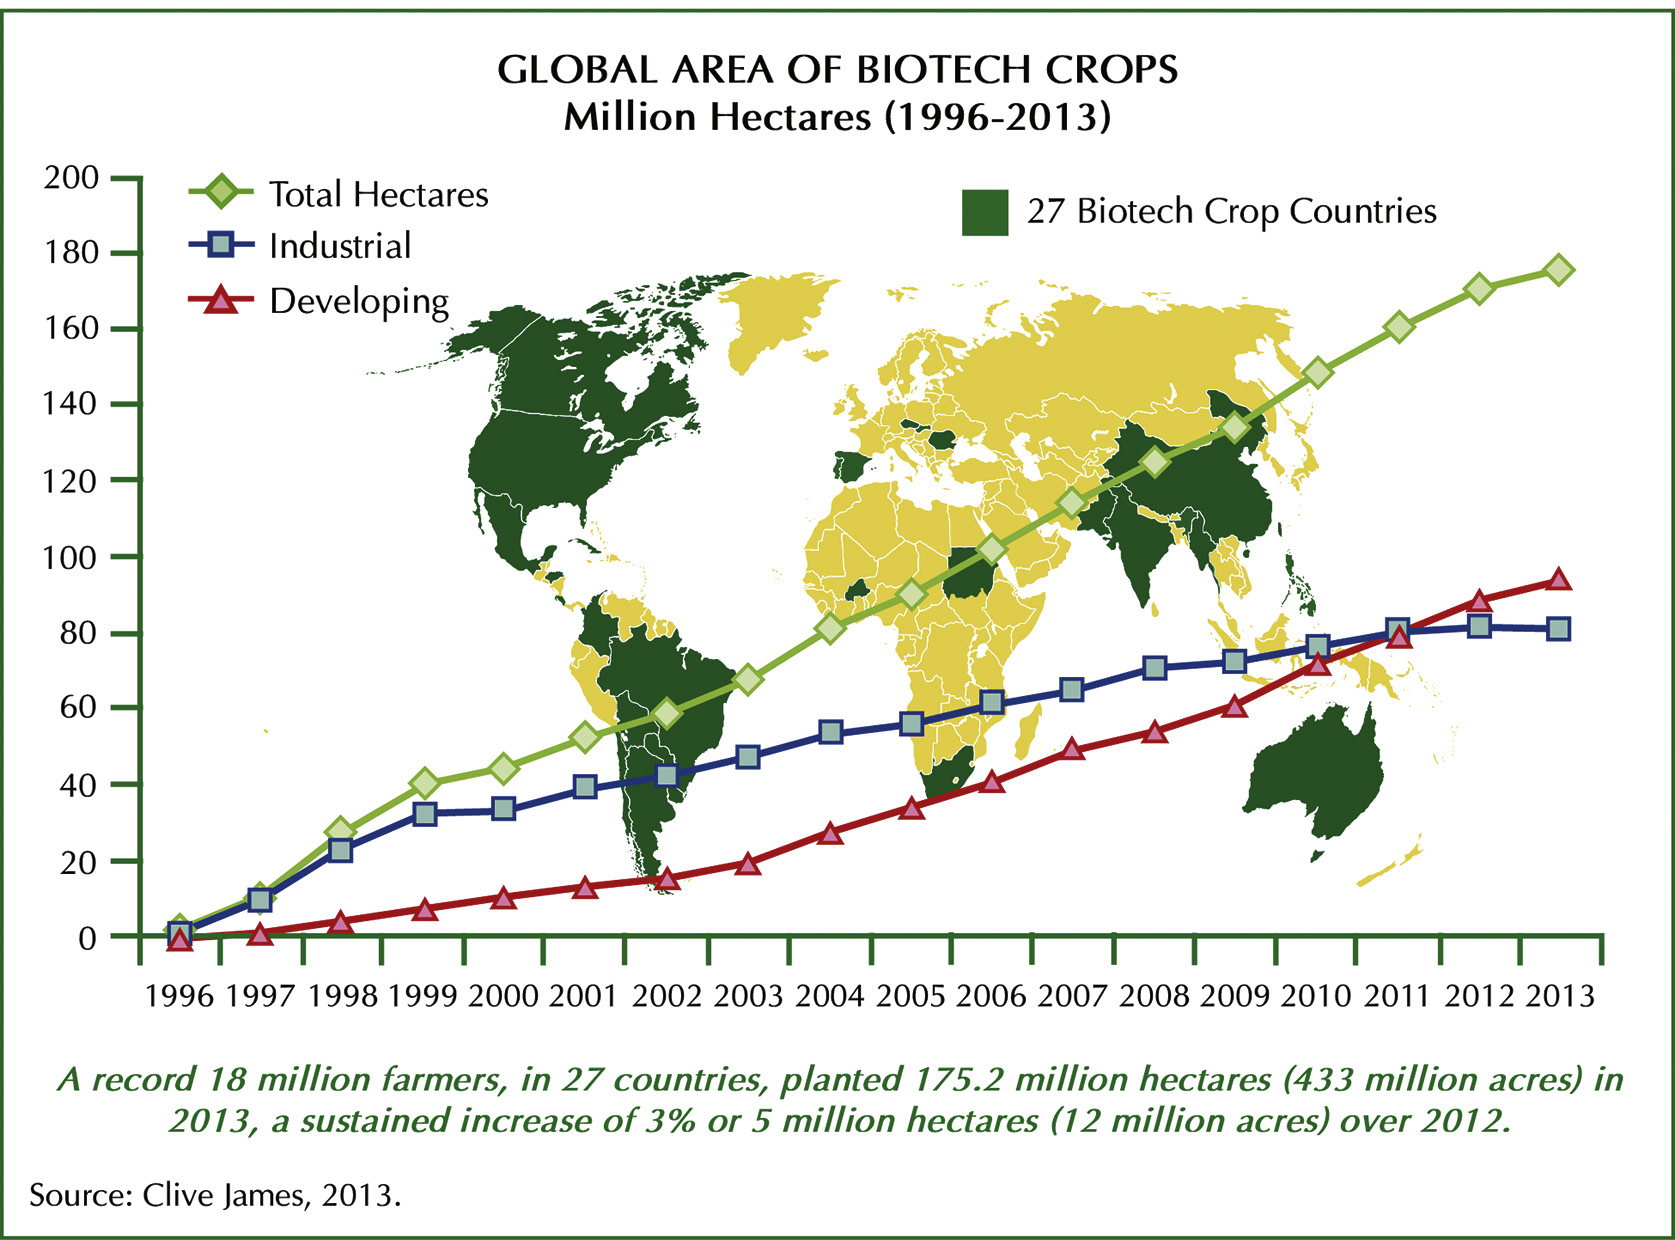
\includegraphics[width=0.4\linewidth]{../images/global_acerage_gmos} \caption{Area of transgenic crops planted worldwide from 1996–2013. From James C (2013). Global Status of Commercialized Biotech/GM Crops for 2013: ISAAA Brief 43. ISAAA, Ithaca, NY.}\label{fig:biotech-crops}
\end{figure}
\end{frame}

\begin{frame}{}
\protect\hypertarget{section}{}
\begin{itemize}
\tightlist
\item
  Worldwide, soybean, maize, canola and cotton have experienced a
  substantial addition of production volume and value with GM crop
  technology.
\item
  Major traits of targets have been herbicide resistance, stacked
  traits, and insect resistance (ISAAA, 2018).

  \begin{itemize}
  \tightlist
  \item
    GM IR crops (\emph{Bt} potato, \emph{Bt} maize, \emph{Bt} cotton)
    account for 12\% of global plantings
  \item
    GM with stacked traits account for 41\% of global plantings
  \item
    GM HT (Bromoxynil herbicide-resistant cotton, glyphosate-resistant
    soybean) crops account for 47\% of global plantings
  \end{itemize}
\end{itemize}

\begin{figure}
\includegraphics[width=0.25\linewidth]{02-introduction_to_plant_biotechnology_files/figure-beamer/biotech-crops-cropwise-2018-1} \caption{Percentage coverage of transgenic crops planted worldwide during 2018}\label{fig:biotech-crops-cropwise-2018}
\end{figure}
\end{frame}

\hypertarget{good-versus-evil}{%
\section{Good versus Evil}\label{good-versus-evil}}

\begin{frame}{Pros}
\protect\hypertarget{pros}{}
\begin{itemize}
\item
  GM crops have contributed to a significant reduction in the global
  environmental impact of production agriculture. Since 1996, the use of
  pesticides was reduced by 503 million kg of AI, constituting an 8.8\%
  reduction, and the overall environmental impact associated with
  pesticide use on these crops was reduced by 18.7\%
\item
  GM IR cotton has contributed a 25.6\% reduction in the volume of AI
  used and a 28.2\% reduction in the EIQ\footnote<.->{An assessment of
    both pesticide active‐ingredient use and the specific pesticides
    used, developed by Kovach et al.~(1992). EIQ value is multiplied by
    the amount of pesticide active ingredient (AI) used per ha to
    produce a field EIQ value. For example, EIQ rating for glyphosate is
    15.3 and EIQ field value for atrazine is 22.9 per hectare} indicator
  (1996--2012)
\item
  GM crops have contributed to reduction in fuel use and cost reduction
  for farmers in cultivation and pest control.
\end{itemize}
\end{frame}

\begin{frame}{}
\protect\hypertarget{section-1}{}
\begin{itemize}
\tightlist
\item
  Abiotic stress tolerance (Maize - 7, sugarcane - 3, soybean - 2).
  Abiotic stresses cause alterations in expression of an array of genes,
  hence adaptation to these require interplay of many gene networks
  (ISAAA, 2019).

  \begin{itemize}
  \tightlist
  \item
    Bacterial cold shock proteins (\emph{csp}, Csp3, CspB) for heat,
    cold and water-deficit stress (CspB has been used in Monsanto's
    drought-tolerant transgenic commercial maize hybrid);
  \item
    Transcription factors (Overexpression of \emph{Hahb}-4, a
    \emph{Helianthus annus} homeobox-leucine zipper gene, which is
    induced by water-deficit conditions and binds to cis-elements of
    genes regulated by dehydration, with a constitutive or its own
    promoter imparts drought tolerance.)
  \end{itemize}
\item
  Development of disease resistant crops (Resistance to Cucumber MV,
  Zucchini YMV, Watermelon mosaic poty virus 2 in \alert{Squash} by
  expression of viral coat protein (cp) gene as transgene; Resistance to
  Papaya ringspot virus using viral coat protein in Papaya)
\item
  Improvement of nutritional quality -- Biofortification.

  \begin{itemize}
  \tightlist
  \item
    Provitamin A biofortified rice (Uses \emph{psy} gene from daffodil
    and \emph{crtI} gene from bacterium, \emph{Erwinia uredovora})
  \item
    Modified lipid content in oilseed crops (18 transgenic events as of
    2019)
  \end{itemize}
\end{itemize}
\end{frame}

\begin{frame}{}
\protect\hypertarget{section-2}{}
\begin{itemize}
\tightlist
\item
  Rapid regeneration of plantlets and propagules using micropropagation.
\item
  Plant and animal disease diagnosis and characterization.
\item
  Rapid gain in crop improvement using molecular marker assisted
  breeding.
\item
  Characterization, conservation and use of germplasm

  \begin{itemize}
  \tightlist
  \item
    DNA fingerprinting
  \item
    Cryopreservation techniques
  \item
    In-vitro regeneration, haploidization
  \end{itemize}
\end{itemize}
\end{frame}

\begin{frame}{Cons}
\protect\hypertarget{cons}{}
\begin{itemize}
\tightlist
\item
  Regards for human health, mostly concerning toxicity and allergenicity
\item
  Indiscriminate use of herbicide and pesticides with possibility for
  resurgence of super-weeds.

  \begin{itemize}
  \tightlist
  \item
    Out of 24 glyphosate-resistant weed species, so far, 16 have been
    reported from transgenic cropping systems (Heap 2014). Amongst them
    \emph{Conyza canadensis} is the most widespread weed plant whilst
    \emph{Amaranthus palmeriand} and \emph{Amaranthus tuberculatus} are
    the two most economically damaging
  \end{itemize}
\item
  Possibility for horizontal transfer of antibiotic-resistant marker
  genes from transgenic food to animal and human gut microbe.
\item
  Plants with improved resistance to drought, disease, or insect pests
  would have an advantage in the wild, and thus, hybridization of
  transgenic crops with wild varieties would be expected to occur.

  \begin{itemize}
  \tightlist
  \item
    Wild maize (corn) in Mexico examined in 2001 contained transgenic
    DNA, even though planting transgenic corn plants was stopped in
    1998!
  \end{itemize}
\end{itemize}
\end{frame}

\hypertarget{biotechnology-its-roots-into-nepal}{%
\section{Biotechnology: Its roots into
Nepal}\label{biotechnology-its-roots-into-nepal}}

\begin{frame}{Research and policy}
\protect\hypertarget{research-and-policy}{}
\begin{itemize}
\tightlist
\item
  Biotechnology policy, 2063

  \begin{itemize}
  \tightlist
  \item
    To increase production and productivity by means of research and
    development of biotechnology as well as transfer of technology, and
    improve the living standard of Nepali people by achieving a
    significant progress in the field of public health and environment
  \end{itemize}
\end{itemize}

\begin{block}{What is biotechnology ?}
\protect\hypertarget{what-is-biotechnology}{}
Accomplishes such a task that channelizes the characteristics and
property of any organism or their living cells/tissues etc. in the work
of human welfare.
\end{block}
\end{frame}

\begin{frame}{Research highlights and project undertakings by NAST}
\protect\hypertarget{research-highlights-and-project-undertakings-by-nast}{}
\footnotesize

\begin{itemize}
\item
  Molecular Characterization and DNA Barcoding of Threatened Flora and
  Fauna of Nepal
\item
  Research on diabetes and obesity emphasizing discovering of a potent
  protein tyrosine phosphatase 1B (PTP1B) inhibitor from the medicinal
  plants of Nepal. PTP1B enzyme plays a paramount role as a negative
  regulator in insulin and leptin signaling pathways that are concerned
  with type 2 diabetes and obesity.
\item
  Ex situ conservation via seed banking for collection and conservation
  of wild plant biodiversity of Nepal and its extension research
  activity. Seeds of wild plant species are collected from different
  forest types of Nepal like tropical to alpine forests. Collected seeds
  thus are curated and conserved under -20 degree C in the seed bank of
  NAST for research, reintroduction and for forest rehabilitation in the
  future.
\item
  PCR-Based Diagnosis of Citrus Huanglongbing Disease in Nepal
\item
  Set facilities in Biotechnology Division, NAST

  \begin{itemize}
  \tightlist
  \item
    Automated DNA Sequencer
  \item
    Tissue lyser
  \item
    Gel Document System
  \item
    Biophotometer
  \item
    SDS PAGE
  \end{itemize}
\end{itemize}
\end{frame}

\hypertarget{use-for-crop-improvement-in-nepal}{%
\section{Use for Crop improvement in
Nepal}\label{use-for-crop-improvement-in-nepal}}

\begin{frame}{Tissue culture/Micropropagation}
\protect\hypertarget{tissue-culturemicropropagation}{}
\begin{figure}
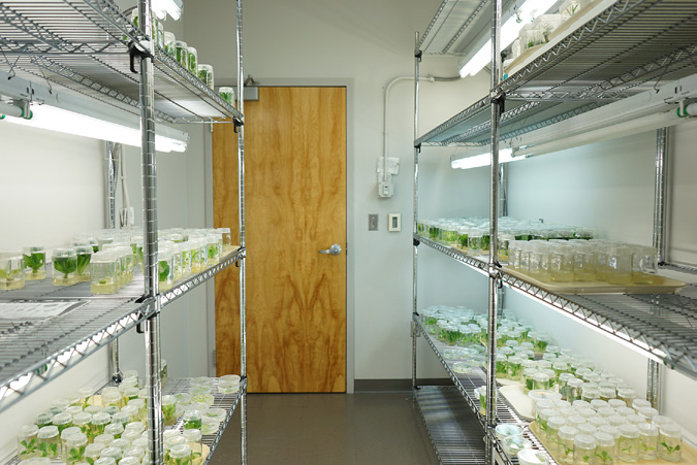
\includegraphics[width=0.6\linewidth]{../images/tissue_culture_chamber} \caption{A walk-in tissue culture growth room with supplementary cooling and shelves with cool white fluorescent lamps}\label{fig:tissue-culture-illustration}
\end{figure}
\end{frame}

\begin{frame}{Molecular tools and application for crop improvement}
\protect\hypertarget{molecular-tools-and-application-for-crop-improvement}{}
\begin{itemize}
\tightlist
\item
  Molecular evaluation and characterization of indigineous as well as
  imported germplasm (maize inbred lines and rice genotypes).
\item
  Rice fungal blast resistance gene screening using molecular markers
\item
  Characterization of maize germplasm using molecular markers
\item
  A QTL for high grain yield under lowland drought in the background of
  popular rice variety Sabitri from Nepal (Study used SSR markers).
  (Yadaw et al. \protect\hyperlink{ref-yadaw2013qtl}{2013})
\item
  Identification and mapping of leaf, stem and stripe rust resistance
  trait loci and their interactions in durum wheat (Study used DArT
  markers). (Singh et al.
  \protect\hyperlink{ref-singh2013identification}{2013})
\item
  Genetic relatedness and population differentiation of Himalayan
  hullless barley (H vulgare L.) landrace inferred with SSRs. (Pandey et
  al. \protect\hyperlink{ref-pandey2006genetic}{2006})
\item
  Deciphering the genetic basis of root morphology, nutrient uptake,
  yield, and yield-related traits in rice under dry direct-seeded
  cultivation systems (Study used GWAS). (Sandhu et al.
  \protect\hyperlink{ref-sandhu2019deciphering}{2019})
\end{itemize}
\end{frame}

\hypertarget{general-use-in-nepal}{%
\section{General use in Nepal}\label{general-use-in-nepal}}

\begin{frame}{}
\protect\hypertarget{section-3}{}
\begin{itemize}
\tightlist
\item
  DFTQC is providing Pesticide Residue Analysis (using RBPR method) and
  microbial testing facilities at several food laboratories and
  quarantine points.
\item
  Prognosis and detection of human/zoonotic pathogens

  \begin{itemize}
  \tightlist
  \item
    As of 6 December, National Pathogen Genetic Sequencing Consortium,
    with support from WHO, an extension of National Public Health
    Laboratory (NPHL) which was set up in March 2021 and grew
    operational in October 2021 has sequenced around 100 genomes of
    SARS-CoV-2.
  \end{itemize}
\item
  Clinical analysis of DNA, RNA, chromosomes and proteins for heritable
  disease diagnosis, prenatal screening and testing of high-risk
  families.
\end{itemize}
\end{frame}

\begin{frame}{}
\protect\hypertarget{section-4}{}
\scriptsize

\begin{figure}
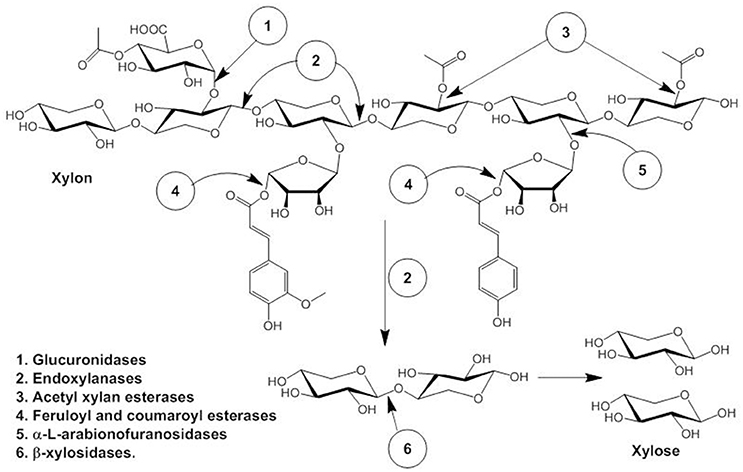
\includegraphics[width=0.65\linewidth]{../images/thermophilic-bacteria-xylanases} \caption{Lignocellulose is mainly obtained from agriculture, horticulture and forest waste, paper-pulp, timber and other agro-forest allied industries. Such lignocelluloses waste can potentially be utilized into various value-added products such as biofuels like bioethanol and biochemical products. Hemicellulose, the second most abundant polysaccharide after cellulose consists of $\beta$-1, 4 linked D-xylopyranosyl units linked with branches of O-acetyl, $\alpha$-L-arabinofuranosyl and $\alpha$-D-glucuronyl residues (La Grange et al., 2001). Synergistic action of several enzymes are required for complete degradation of hemicellulose to pentose sugar, namely endoxylanases (endo-$\beta$- 1,4-xylanase), $\beta$-xylosidases (xylan 1,4-$\beta$-xylosidase), and $\alpha$- glucuronidases ($\alpha$-glucosiduronase) and side-chain cleaving enzymes: $\alpha$-L-arabinofuranosidase, feruloyl esterase, and acetyl xylan esterase that produces xylooligomers which are further degraded to monomeric sugar xylose by $\beta$-D-xylosidases. \textbf{Production, Purification, and Characterization of Thermostable Alkaline Xylanase From Anoxybacillus kamchatkensis (Paudwar Hot Springs, Myagdi, Nepal) NASTPD13 (can be cultured at a range of 37-75 degree C temperature, pH 7)}.}\label{fig:xylanase-production-purification-nepal}
\end{figure}
\end{frame}

\begin{frame}{}
\protect\hypertarget{section-5}{}
\begin{figure}
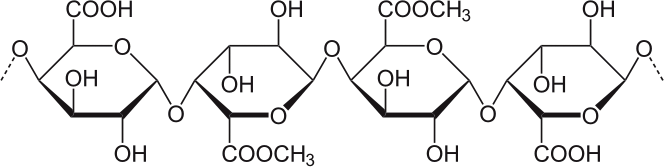
\includegraphics[width=0.65\linewidth]{../images/pectin-chemical-structure} \caption{Pectinase enzymes are classified into polygalcturonase(PG), pectinesterase(PE), and pectin lyase(PL) based on their mode of action on the substrate (Jayani et al. 2005). Pectinase enzymes are extensively used in an industrial sector especially in food industry i.e. fruit juice extraction, coffee and tea fermentation, oil extraction, improvement of chromaticity and stability of red wine (Jayani et al. 2005). Besides food industry; pectinases are widely used in textile, paper and pulp industries, waste-water treatment (Solbak et al. 2005; Ahlawat et al. 2014). More recently, the enzyme has been used with cellulose enzyme for the production bioethanol from lignocellulosic biomass. \textbf{Alkaline thermostable pectinase enzyme from Aspergillus niger strain MCAS2 isolated from Manaslu Conservation Area, Gorkha, Nepal}}\label{fig:pectinase-isolation-nepal}
\end{figure}
\end{frame}

\hypertarget{ethical-biotechnology}{%
\section{Ethical biotechnology}\label{ethical-biotechnology}}

\begin{frame}{Biotechnology whims: A case of mosquito control in
Florida, US}
\protect\hypertarget{biotechnology-whims-a-case-of-mosquito-control-in-florida-us}{}
\footnotesize

Local officials in Florida have approved the release of 750 million
mosquitoes that have been genetically modified to reduce local
populations. The aim is to reduce the number of mosquitoes that carry
diseases like dengue or the Zika virus.

The green-lighting of a pilot project after years of debate drew a swift
outcry from environmental groups, who warned of unintended consequences.
Activists warn of possible damage to ecosystems, and the potential
creation of hybrid, insecticide-resistant mosquitoes.

But the company involved says there will be no adverse risk to humans or
the environment, and points to a slate of government-backed studies.
Aedes aegypti mosquitoes are known to spread deadly diseases to humans
such as dengue, Zika, chikungunya, and yellow fever.

Only female mosquitoes bite humans because they need blood to produce
eggs. So the plan is to release the male, modified mosquitoes who will
then hopefully breed with wild female mosquitoes. However, the males
carry a protein that will kill off any female offspring before they
reach mature biting age. Males, which only feed on nectar, will survive
and pass on the genes\footnote<.->{\url{https://www.bbc.com/news/world-us-canada-53856776}}.
\end{frame}

\hypertarget{bibliography}{%
\section{Bibliography}\label{bibliography}}

\begin{frame}{References}
\protect\hypertarget{references}{}
\hypertarget{refs}{}
\begin{cslreferences}
\leavevmode\hypertarget{ref-klumper2014meta}{}%
Klümper, Wilhelm, and Matin Qaim. 2014. ``A Meta-Analysis of the Impacts
of Genetically Modified Crops.'' \emph{PloS One} 9 (11): e111629.

\leavevmode\hypertarget{ref-pandey2006genetic}{}%
Pandey, Madhav, Carola Wagner, Wolfgang Friedt, and Frank Ordon. 2006.
``Genetic Relatedness and Population Differentiation of Himalayan
Hulless Barley (Hordeum Vulgare L.) Landraces Inferred with Ssrs.''
\emph{Theoretical and Applied Genetics} 113 (4): 715--29.

\leavevmode\hypertarget{ref-sandhu2019deciphering}{}%
Sandhu, Nitika, Sushil Raj Subedi, Vikas Kumar Singh, Pallavi Sinha,
Santosh Kumar, SP Singh, Surya Kant Ghimire, et al. 2019. ``Deciphering
the Genetic Basis of Root Morphology, Nutrient Uptake, Yield, and
Yield-Related Traits in Rice Under Dry Direct-Seeded Cultivation
Systems.'' \emph{Scientific Reports} 9 (1): 1--16.

\leavevmode\hypertarget{ref-singh2013identification}{}%
Singh, A, MP Pandey, AK Singh, RE Knox, K Ammar, JM Clarke, FR Clarke,
et al. 2013. ``Identification and Mapping of Leaf, Stem and Stripe Rust
Resistance Quantitative Trait Loci and Their Interactions in Durum
Wheat.'' \emph{Molecular Breeding} 31 (2): 405--18.

\leavevmode\hypertarget{ref-yadaw2013qtl}{}%
Yadaw, Ram Baran, Shalabh Dixit, Anitha Raman, Krishna Kumar Mishra,
Prashant Vikram, BP Mallikarjuna Swamy, Ma Teresa Sta Cruz, Paul T
Maturan, Madhav Pandey, and Arvind Kumar. 2013. ``A Qtl for High Grain
Yield Under Lowland Drought in the Background of Popular Rice Variety
Sabitri from Nepal.'' \emph{Field Crops Research} 144: 281--87.
\end{cslreferences}
\end{frame}

\end{document}
